\section{Intervention}
\label{sec:method}

To ensure a fair comparison, all conditions share the same three agents,
interaction order (Planner, then Executor, then Reviewer), message-passing
graph, agent-call budget and ground-truth evaluator, and, outside
enforcement, the same context visibility. All use greedy decoding at temperature $0$ and stop a trajectory at its
first PASS. How often a team calls the evaluator, by contrast, is an outcome of its
organization (\S\ref{subsec:mechanism}). Apart from the role instructions
themselves, the conditions differ in two respects. First, the repair hint
that follows a FAIL, written with the gold answer in view and instructed
not to reveal it, reaches the role-structured and enforced teams through
each role's advice slot, the template field reserved for feedback, and the
role-free team as an entry in its shared history
(Figure~\ref{fig:pipeline}). Second, the role-free prompt's closing instruction, its footer, asks
every agent for an answer.

\begin{figure}[t]
\centering
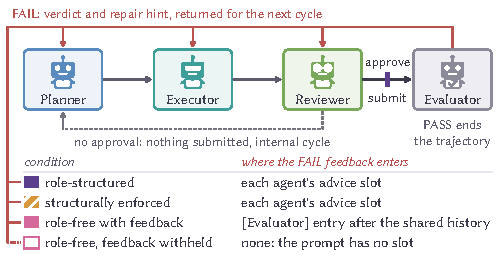
\includegraphics[width=0.585\textwidth]{figures/fig_pipeline.pdf}
\caption{\textbf{One deliberation cycle and where the feedback enters.}
A trajectory (one problem's run, at most six cycles) advances one cycle per
pass of Planner, Executor and Reviewer. The third agent's approval (the bar)
is the only route to the evaluator, which knows the reference answer and
returns a verdict: PASS, ending
the trajectory, or FAIL with a repair hint; without approval the team
deliberates internally in the next cycle. A trajectory that never submits
is graded once (one verdict) when the budget runs out.}
\label{fig:pipeline}
\end{figure}

\paragraph{Role-structured \PER{} (baseline).} Role prompts are as ordinarily written. The Reviewer is instructed to approve only a
complete answer of the expected form and, in a cycle that receives a FAIL,
to route the work back to the Planner or Executor instead of approving.

\paragraph{Role-free with feedback (main comparison).} Every clause that
assigns a function is removed, including the Planner's \textsc{must not}s
and the Reviewer's two clauses on approval. All three agents receive one
identical prompt, ``You are one of three agents collaboratively solving
this problem. Continue the work.'', followed by the problem, the shared history and
the agent's position. The footer asks for its current best answer and a decision to
submit or to keep deliberating. Outside structural enforcement, the third agent's decision to submit is
the team's approval. After a FAIL, all three agents see the verdict and hint as a
shared entry for one cycle, so the two teams have equal access to external
feedback; how many verdicts each draws depends on its submissions.

\paragraph{Role-free, feedback withheld (diagnostic).} The role-free prompt
minus the evaluator's entry shows what a role ablation measures when it
also removes the feedback channel.

\paragraph{Structurally enforced.} Here the interface, not the prompt
wording, enforces specialization. The Planner outputs JSON against a schema
without an answer field, so a final answer is unrepresentable. The Executor receives only the parsed plan, not the
Planner's text, and the Reviewer's acceptance promotes the
Executor's answer by reference. A trajectory terminates when malformed
outputs exhaust the allowed regenerations (Appendix~\ref{app:details}).

\subsection{Pre-registered and exploratory analyses}
\label{subsec:prereg}

We fixed all five pre-specified endpoints (P1 to P5) in writing before
collecting any intervention data. Every test is paired at the problem
level: significance is the exact McNemar test~\cite{mcnemar1947note} on
discordant pairs (problems that exactly one condition gets right), and
bootstrap intervals resample whole problems~\cite{efron1979bootstrap}.
Trajectories that never produce a graded answer count as incorrect, except
in the first-pass contrast. The pre-registered primary endpoint, P4, which
asks whether enforcement's effect on accuracy varies by actor, is null after Holm's correction~\cite{holm1979simple}. We added the role-free condition with feedback, and with it the
main comparison, after the freeze, when the dataset and analysis plan were
fixed. Its design and primary analysis were committed in writing before
any of its data existed, but we classify its results, like those of the
forced-submission run, as exploratory. Appendix~\ref{sec:prereg} details
all endpoints.
